\section{Experimental Evaluation}\label{sec:experiments}
We now describe the experiments to be conducted for this study.
The goals for our experiments is to understand the performance characteristics of queries with and without pipelining. 
We conduct our experiments in \sys{}, an in-memory database engine. 
%We describe the proposed methodology below. 

\subsection{Workload}
We use queries and dataset from the TPC-H benchmark~\cite{tpc-h} for scale factor 50.

%We perform an analysis of the TPC-H queries based on how they are impacted by pipelining. 
%Note that the analysis uses query plans generated by \sys{}'s cost based query optimizer. 

We acknowledge that systems may differ based on their cost models, heuristics and general query optimization techniques.
\sys{} uses hash based implementation of join algorithms, which makes a pipeline of (selection operator $\rightarrow$ probe operator) possible. 
Other systems may produce query plans with different pipelines than those in \sys{}. 
Therefore the results for pipelining analysis for \sys{} may not be the same for other systems.
However the methodology used for our analysis should be broadly applicable for different systems as well as workloads other than TPC-H. 

\begin{figure*}[ht]
	\centering 
	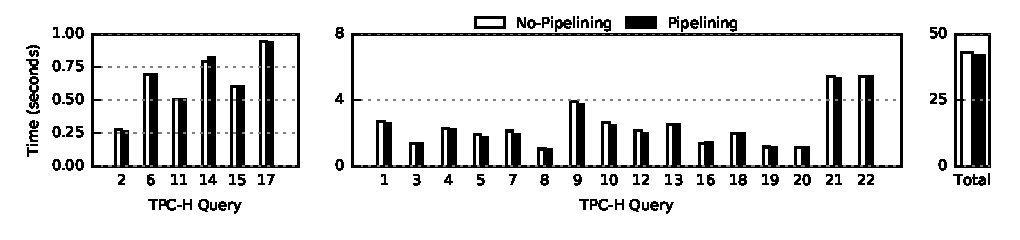
\includegraphics{pipeline/figures/colstore-20threads-bs2mb-withlip-alltpch}
	\caption{\textbf{Execution times of TPC-H queries with base tables in column store format and block size 2 MB}}
	\label{fig:absolute-times-all-tpch-bs2mb-20threads}
\end{figure*}

\subsection{Hardware Description}\label{ssec:hardware-description}
We now describe the hardware configuration and \sys{} specifications used for our evaluation. 
The hardware configuration of the machine that we used are described in Table~\ref{table:hardware}.

\begin{table}[h]
	\centering
	\begin{tabular}{|p{0.62in}|p{2.4in}|}
		\hline
		\textbf{Parameter} & \textbf{Description} \\ \hline
		Processor & 2 Intel Xeon Intel E5-2660 v3 2.60 GHz (Haswell EP) processors\\ \hline
		Cores & 10 physical, 20 with hyper-threading per socket \\ \hline
		Memory & 80 GB per NUMA socket, 160 GB total \\ \hline
		Caches & L3: 25 MB, L2: 256 KB, L1 (both instruction and data): 32 KB \\ \hline
		OS & Ubuntu 14.04.1 LTS \\ \hline
	\end{tabular}
	\caption{\textbf{Evaluation platform}}
	\label{table:hardware}
\end{table}

Our analysis focuses on performance of single socket, and thus we use only one of the two NUMA sockets on the machine.
Unless specified, we use all 20 threads as \sys{} workers.
The buffer pool size of \sys{} is configured with 80\% of the system's memory viz. 126 GB.
We run each query 11 times, discard the first two runs and report the median of the remaining nine runs. 
%We perform hardware instrumentation using Processor Counter Monitor (PCM) library~\cite{pcm}.

%Hence we do not consider such queries for our study (Q11, Q12, Q17 \todo{verify}).

%A good candidate for our pipeline study is a query that has a large input to the pipeline and has significant amount of data gets passed through the pipeline. 

\begin{figure}[ht]
	\centering 
	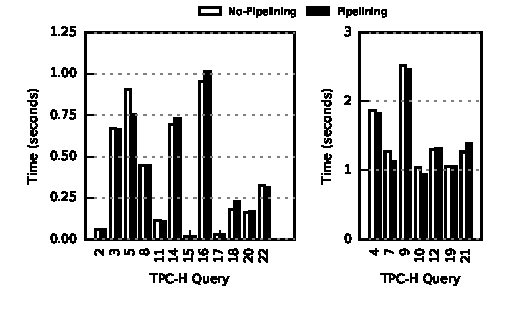
\includegraphics{pipeline/figures/deep-pipeline-comparison-2mb-withlip}
	\caption{\textbf{Execution times of operator pipelines in TPC-H query plans using pipelining and non-pipelining strategies with block size 2 MB}}
	\label{fig:deep-pipeline-comparison-2mb}
\end{figure}

\subsection{Results}
In this section we discuss the results of our experimental evaluation. 
We focus on the following metrics: Overall query response time, execution time of a pipeline, and execution time of individual operator \wo{}s.

\begin{figure*}[t]
	\centering
	\begin{subfigure}[ht]{0.32\textwidth}
		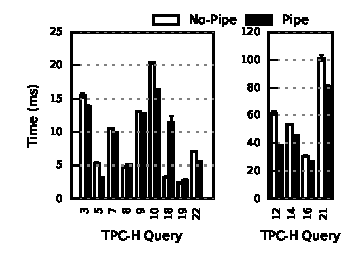
\includegraphics[width=\textwidth]{pipeline/figures/first-consumer-comparison-1mb-withlip}	
		\caption{Block size 1 MB}
	\end{subfigure}
	~
	\begin{subfigure}[ht]{0.32\textwidth}
		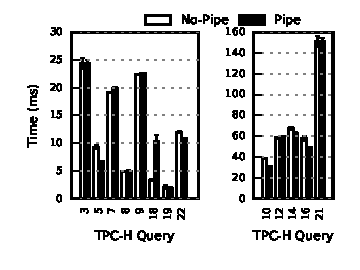
\includegraphics[width=\textwidth]{pipeline/figures/first-consumer-comparison-2mb-withlip}	
		\caption{Block size 2 MB}		
	\end{subfigure}
	~
	\begin{subfigure}[ht]{0.32\textwidth}
		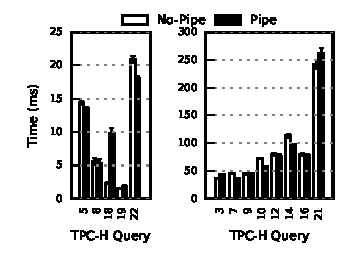
\includegraphics[width=\textwidth]{pipeline/figures/first-consumer-comparison-4mb-withlip}	
		\caption{Block size 4 MB}
	\end{subfigure}
	\caption{\textbf{Performance comparison of probe hash operator when it is the first consumer operator in a pipeline}}
	\label{fig:first-consumer-comparison}
\end{figure*}

\subsubsection{Impact of pipelining on query performance}
We are interested in measuring the impact of pipelining on a query's performance.
The only observable metric for a user of the system is the response time of a query.
Complex queries like the ones in TPC-H are made up of several pipelining consisting of multiple operators.
Thus it is not immediately clear of the impact of pipelining on the entire query's response time. 
We claim that not all queries benefit from pipelining equally.

To understand the impact of pipelining on a query's response time, we first try to understand where does time go in a TPC-H query execution.
%Pipelining typically improves the performance of the consumer operator(s) in a pipeline. 
The intuition is that if there is only one operator in the query where majority of the query execution time is spent, pipelining may not play a big role in the overall execution time of the query.
To make the analysis simpler, we analyze the most dominant operator (where the highest time is spent) and the second most dominant operator. 
Note that for this analysis, we run the queries in the non-pipelining mode, so that the percent time spent metric is accurate.

Figure~\ref{fig:time-distribution-all-tpch-colstore} shows the results of this experiment, for tables stored in column store format. 
For some queries (Q1, Q6, Q13, Q15, Q17, Q19, Q22) the dominant operator takes up the majority of the query execution time (more than 50\%).
We also note that the dominant operator for many of these queries is a leaf operator (e.g. Selection on a base table, building a hash table on a base table, Aggregation on a base table). 
Thus, these queries may not really get benefits from the pipelining by the virtue of their query plan structures.

In many queries even though there are pipelines of operators, majority of the data is pruned out at the base of the pipeline. 
Therefore not enough data is passed on to the consumer operators and hence the impact of pipelining is minimal. 

\subsubsection{Performance of Consumer Operator}
Pipelining should benefit the consumer operator as its input should be hot in caches.
To verify if pipelining improves the performance of the consumer operator, we perform the following experiment.

We compare the \wo{} execution time for the deepest pipelines in which the first consumer operator is a probe operator for a join.
If there are multiple deep pipelines in a query with equal length, we pick the pipeline that has more number of tasks at the starting operator. 
The reason we pick probe hash table operator is that selection $\rightarrow$ probe pipeline is commonly found in query plans.
To reduce noise, we consider only such probe operators for which there are at least 5 \wo{}s.

We can observe in Figure~\ref{fig:first-consumer-comparison} that in general pipelining benefits the performance of the performance of the probe operator. 
The extent of improvement diminishes as we increase the block size from 1 MB to 4 MB.
%Moreover the performance improvement due to pipelining does not result into improvement in the overall query execution times.

\subsubsection{Performance of Deep Pipelines}
Having looked at the performance of the consumer opertors, we zoom out to examine the performance of pipelines in each query.
To do that, we measure the execution time of the deepest pipelines from each query.
The execution time of a pipeline is defined as the time difference between two events: end of execution of the last \wo{} of the last operator in the pipeline and beginning of the execution of the first \wo{} of the first operator in the pipeline. 
Figure~\ref{fig:deep-pipeline-comparison-2mb} shows the results of this experiment. 

Recall that the pipelines in consideration are ones which are deep and the first operator in these pipelines has large amount of work.
Hence these pipelines form a significant fraction of the total query execution time.
We can observe from Figure~\ref{fig:deep-pipeline-comparison-2mb} that the pipeline execution times in the pipelining and non-pipelining implementation are fairly similar, despite some individual consumer operator getting performance improvement due to pipelining (c.f. Figure~\ref{fig:first-consumer-comparison}). 
%That explains why the total execution times of queries shown in Figure~\ref{fig:absolute-times-all-tpch-bs2mb-20threads} are quite similar. 

\subsubsection{Overall Execution Time:}\label{ssec:overall-execution-time} 
After analyzing the performance of deep pipelines, we further zoom out to look at the overall execution times of the queries. 
We compare the overall execution time of queries using pipelining and non-pipelining strategies. 
We use column store storage format for base tables and use a block size of 2 MB for stored tables and temporary tables.

The absolute times for all TPC-H queries for block size 2 MB are shown in Figure ~\ref{fig:absolute-times-all-tpch-bs2mb-20threads}.
We can observe that there is little to no difference between query execution times for pipelining and non-pipelining strategies. 

From these experiments we can conclude that pipelining though benefits individual operators in a query, the overall impact of the choice of with and without pipelining is fairly minimal.

\subsubsection{Effect of Storage Format}
Next we study the effect of storage format of base tables on the pipelining performance. 
We use two configurations: a) All TPC-H tables stored in row store format b) All TPC-H tables stored in column store format. 
Then we compare the improvement of pipelining over non-pipelining for each configuration. 
Note that in both configurations, temporary tables are stored in row store format. 
We run the queries using 20 threads and block size of 2 MB.

\begin{figure*}[ht]
	\centering
	\begin{subfigure}[ht]{0.48\textwidth}
		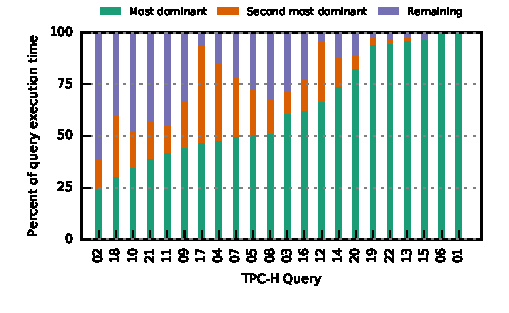
\includegraphics{pipeline/figures/all-tpch-queries-time-distribution-rowstore}
		\caption{\textbf{Row store}}
		\label{fig:time-distribution-all-tpch-rowstore}
	\end{subfigure}
	~
	\begin{subfigure}[ht]{0.48\textwidth}
		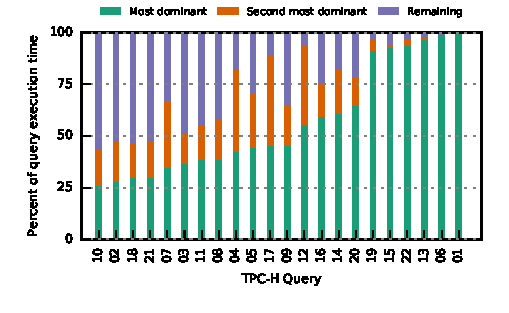
\includegraphics{pipeline/figures/all-tpch-queries-time-distribution-withlip}
		\caption{\textbf{Column store}}
		\label{fig:time-distribution-all-tpch-colstore}
	\end{subfigure}
	\caption{\textbf{Distribution of time spent in each TPC-H query among its operators}}
	\label{fig:tpch-operator-time-distribution}
\end{figure*}


Let us start by understanding the time distribution across operators when we use the row store format.
We present the time distribution for the row store format in Figure~\ref{fig:time-distribution-all-tpch-rowstore}.
Contrast with column store (similar distribution for column store is presented in Figure~\ref{fig:time-distribution-all-tpch-colstore}), we can observe that the dominance of the selection operation on the overall query execution time is higher in case of row store, e.g. Q03, Q07, Q10, Q11, Q12, Q14, Q16, Q18, Q19, Q20.
As a result, we expect that the impact of pipelining on overall query execution time should further diminish when using the row store format.

\begin{figure*}
	\centering 
	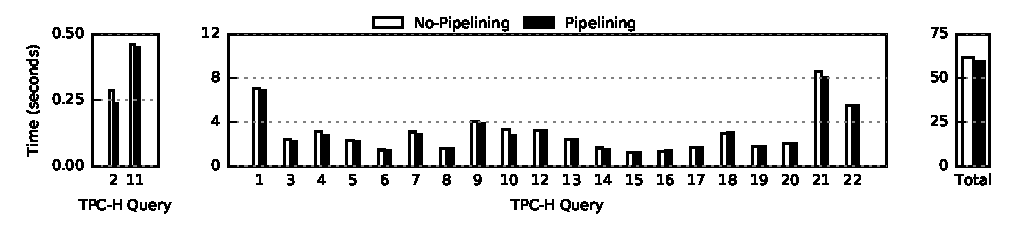
\includegraphics{pipeline/figures/rowstore-20threads-bs2mb-withlip-alltpch}
	\caption{\textbf{Execution times of TPC-H queries with base tables using row store format and block size of 2 MB}}
	\label{fig:absolute-times-all-tpch-bs2mb-20threads-rowstore}
\end{figure*}

We plot the absolute execution times Figure~\ref{fig:absolute-times-all-tpch-bs2mb-20threads-rowstore}.
First, we can observe that column store queries are slightly faster than their row store counterparts. 
Second, the total query execution time is not significantly different between using pipelining and non-pipelining strategy. 

Note that query plans start with accessing base tables in the leaf nodes. 
Base tables usually have more number of columns as compared to the intermediate tables, due to projections.
As we progress upwards (from leaf to root nodes), the number of referenced columns keep decreasing. 
Thus the performance gap for operations on intermediate tables is narrow when using row store vs column store formats.

\subsubsection{Effect of Parallelism}\label{sssec:parallelism-effect}
Next, we study the effect of parallelism on the performance of pipelining and non-pipelining strategies. 
We run the TPC-H queries with 10 threads (instead of the 20 threads used for other experiments) and observe that the relative performance of pipelining and non-pipelining remains similar. 
Hence we don't report the results for experiments with 10 threads.

\begin{figure}[t]
	\centering 
	\begin{subfigure}[ht]{0.225\textwidth}
		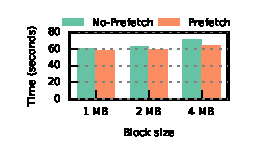
\includegraphics[width=\textwidth]{pipeline/figures/prefetching-total-execution-time-withlip-rowstore}
		\caption{TPC-H execution time}
		\label{fig:prefetching-total}
	\end{subfigure}
	~
	\begin{subfigure}[ht]{0.225\textwidth}
		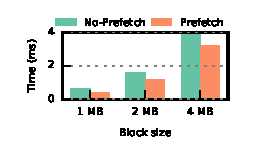
\includegraphics[width=\textwidth]{pipeline/figures/prefetching-q07-select-withlip-rowstore}
		\caption{Q07 selection on \textit{lineitem}}
		\label{fig:prefetching-select-q07}
		\end{subfigure}
		%
	\begin{subfigure}[ht]{0.225\textwidth}
		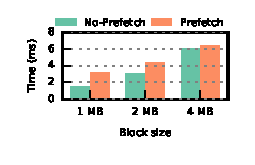
\includegraphics[width=\textwidth]{pipeline/figures/prefetching-q07-build-withlip-rowstore}
		\caption{Q07 build hash on \textit{orders}}
		\label{fig:prefetching-build-q07}
	\end{subfigure}
	~
	\begin{subfigure}[ht]{0.225\textwidth}
		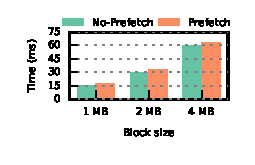
\includegraphics[width=\textwidth]{pipeline/figures/prefetching-q07-probe-withlip-rowstore}
		\caption{Q07 probe hash table}
		\label{fig:prefetching-probe-q07}
	\end{subfigure}
	\caption{\textbf{Performance of row store format with and without hardware prefetching. Shown above are total TPC-H execution times and median \wo{} execution times for selection, probe and build hash operators in Q07 with various block sizes}}
	\label{fig:prefetching-vs-noprefetching-rowstore}
\end{figure}

We present a result from TPC-H Q07 that shows the impact of scalability of operators on the performance of pipelining and non-pipelining strategies.
In TPC-H Q07, there are three probe operators.
One of these probe operators involves probing a large hash table, which is constructed on entire \textit{orders} table without any filter.
The other hash tables in the query plan are relatively smaller. 
As described in Section~\ref{sssec:scalability}, the degree of parallelism (DOP) of an operator in a pipeline is usually lower in the pipelining strategy.

\begin{figure}[ht]
	\centering
	\begin{subfigure}[ht]{0.48\columnwidth}
		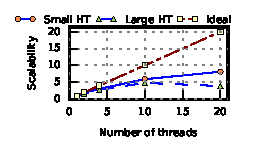
\includegraphics[]{pipeline/figures/tpch-q07-sf50-probe-scalability}	
		\caption{Scalability}
		\label{fig:scalability-tpch-q07}
	\end{subfigure}
	~
	\begin{subfigure}[ht]{0.48\columnwidth}
		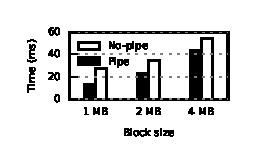
\includegraphics[]{pipeline/figures/scalability-impact-tpchq07-op9-performance}	
		\caption{Execution time}		
		\label{fig:scalability-tpch-q07-exec-times}
	\end{subfigure}
	\caption{\textbf{Scalability of two different probe operators in TPC-H Q07, compared with the ideal scalability. Also shown are the execution times for the probe operator with poor scalability in various settings}}
	\label{fig:scalability-plots}
\end{figure}

We find the scalability of these operators and present them in Figure~\ref{fig:scalability-tpch-q07}.
Note that though the probe operator with smaller hash table (marker {\color{PlotOrange}\FilledSmallCircle}) has less than ideal scalability, it still gives some performance improvement as the number of threads increase.
For the probe operator with large hash table size (marker {\color{PlotGreen}\FilledSmallTriangleUp}), the scalability curve dips as the number of threads increase.
Therefore for this operator, increasing parallelism beyond a limit hurts its performance. 
The reason for the poor scalability of this operator is due to the large size of its probe hash table, because of which there is a large random read traffic during the tuple reconstruction phase of the probe operator. 

To verify if our hypothesis regarding the impact of poor scalability on pipelining and non-pipelining (c.f. Section~\ref{sssec:scalability}) is correct, we compare the median \wo{} execution time for the probe operator with poor scalability in pipelined and non-pipelined implementations.
Figure~\ref{fig:scalability-tpch-q07-exec-times} presents the result of this comparison. 
We can see that the median execution times for pipelining version are lower than that in non-pipelining version in all three block sizes.
The difference between the two times are higher for lower block size and it reduces as the block size increases.
For lower block sizes, the number of probe \wo{}s are higher resulting in a larger contention which causes higher performance degradation.

This behavior leads us to the next question: What is the impact of poor scalability on TPC-H Q07's performance?
The percent improvements of pipelining over non-pipelining in TPC-H Q07's execution times for different block sizes are 20\% (1 MB), 12\% (2 MB), and 9\% (4 MB).
The improvement depends on the position of the poorly scalable operator in a deep pipeline.
If the operator is at the end of the pipeline with less work to be done (compared to the operators at the beginning of the pipeline), the extent of overall query time improvement is low. 

This experiment highlights an aspect of parallelism which causes performance difference between pipelining and non-pipelining strategies.
Systems can have scalability issues due to various external (hardware interference, slow network) and internal factors (skew, poor implementation of operators).
We would like to stress that the reason for poor scalability of the probe operator in \sys{} when the build side is large, is not our focus\footnote{The specific probe operator in TPC-H Q07 can be made more scalable by partitioning the join or by putting the payload in the hash table bucket.}, rather it is the impact of poor scalability on the performance of pipelining strategies.

\subsubsection{Effect of Hardware Prefetching}
We examine the effect of prefetching on the relative performance of pipelining strategy. 
We run this experiment using row store format and use three values for block sizes namely 1 MB, 2 MB and 4 MB.
Figure~\ref{fig:prefetching-vs-noprefetching-rowstore} presents the improvements in query execution times due to hardware prefetching. 
%\todo{What about non-pipelining results?}

In the row store format, even if a single attribute is scanned, a lot of unnecessary data from the tuple is read.
As row store tuples are fixed width\footnote{variable length attributes are stored in a separate region, with a pointer to the region stored in the tuple}, the hardware prefetcher can detect the access pattern of scanning a single attribute. 
We observe that hardware prefetching has a small impact on the total execution time, as shown in Figure~\ref{fig:prefetching-total}. 
Notice that the impact of prefetching on the total execution time increases as the block size increases. 
For a higher block size, the prefetcher can observe more data traffic per block and thus it can speculate and prefetch more efficiently. 

Beyond the overall execution time, we are interested in understanding the impact of hardware prefetching on individual operators. 
We pick three operations namely selection (filter), building a hash table and probing a hash table from TPC-H Q07.
For these operators, we compare there execution time in Figure~\ref{fig:prefetching-select-q07}, Figure~\ref{fig:prefetching-build-q07}, and Figure~\ref{fig:prefetching-probe-q07}.

Our observations are as follows:
Prefetching generally benefits selection operators. 
The extent of improvement increases as the block size increases. 
This behavior is understandable as selection has a sequential access pattern and the prefetcher can understand the strides in the memory accesses across tuples in the row store format.

Prefetching seems to have no impact on probe hash table operator.
A probe operation involves reading two data streams - a sequential read access pattern for the probe input and a random read access pattern for the hash table. 
Perhaps due to a mix of these two access patterns, probe operator does not seem to be benefited by hardware prefetching. 

For the build hash table operation, prefetching seems to have an adverse effect as its \wo{}s get slower with prefetching.
A possible explanation for this slowdown could be the mixed access patterns of sequential read and random write behavior in the build hash operation.

An interesting direction for future work would be to perform controlled experiments to understand the effect 
of prefetching on the performance of hash-based joins.

\begin{figure*}[ht]
	\centering
	\begin{subfigure}[ht]{0.3\textwidth}
		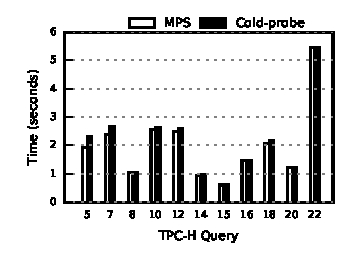
\includegraphics[width=\textwidth]{pipeline/figures/coldprobe-sequence-20threads-tpch-sf50-bs1mb-withlip-colstore}	
		\caption{Block size 1 MB}
	\end{subfigure}
	~
	\begin{subfigure}[ht]{0.3\textwidth}
		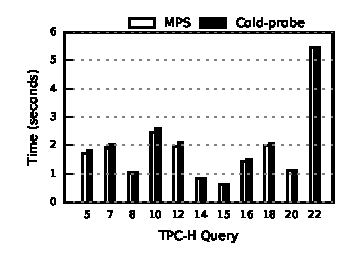
\includegraphics[width=\textwidth]{pipeline/figures/coldprobe-sequence-20threads-tpch-sf50-bs2mb-withlip-colstore}	
		\caption{Block size 2 MB}
	\end{subfigure}
	~
	\begin{subfigure}[ht]{0.3\textwidth}
		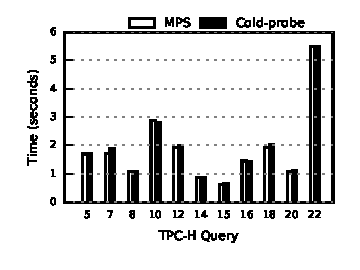
\includegraphics[width=\textwidth]{pipeline/figures/coldprobe-sequence-20threads-tpch-sf50-bs4mb-withlip-colstore}	
		\caption{Block size 4 MB}
	\end{subfigure}
	\caption{\textbf{Comparison of query performances that use two different pipeline sequences. MPS refers to the pipeline sequence output by the MPS algorithm proposed in Section~\ref{ssec:pipeline-sequencing-algo} and another sequence in which probe input is cold, but the hash table is hot at the time of first probe}}
	\label{fig:pipeline-sequence-comparison}
\end{figure*}

We ran the same experiment for column store format and found little to no performance difference due to prefetching. 
We speculate that the prefetcher does not make any significant contribution to an already optimized access pattern of column stores.
\begin{figure}[ht]
	\centering 
	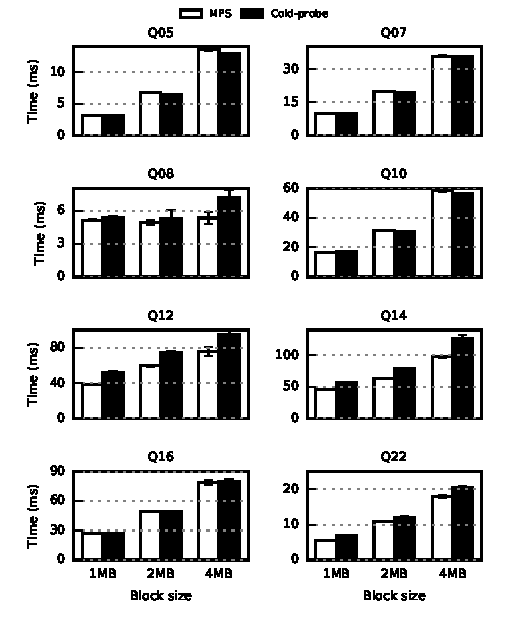
\includegraphics{pipeline/figures/first-probe-comparison-mps-vs-coldprobe-20threads-colstore-withlip}
	\caption{\textbf{Probe performance in cold probe sequence vs MPS algorithm output}}
	\label{fig:coldprobe-vs-mps}
\end{figure}

\subsection{Effect of Pipeline Sequences}
We now evaluate the effect of using different sequences of pipelines in a query plan. 
Note that some TPC-H queries have a large plan (e.g. Q07, Q21), in which there can be several such sequences possible.
On the flipside, plans for some queries are so small such that we cannot produce multiple pipeline sequences (e.g. Q01, Q06).
Thus to keep our analysis manageable, we produce pipeline sequences which can be given a semantic information. 
One such sequence is the output of the MPS algorithm proposed in Section~\ref{ssec:pipeline-sequencing-algo}.
Recall that the heuristics for the MPS algorithm was to produce a maximal probe pipeline, in which the probe input would be hot in caches, as much as possible.
We use another sequence in which the probe input is cold, however the hash table is hot. 

We use the following criterion for selecting a query for this experiment:
We should come up with multiple pipeline sequences from the given query plan.
In the deepest pipeline, there should be a probe operator whose input is not a stored table, and the input itself should have substantial (at least 10 \wo{}s). 

In all the previous experiments, we use the pipeline sequence which is an output of the MPS algorithm. 
Thus we only show the results for the cold probe sequence in Figure~\ref{fig:pipeline-sequence-comparison}. 
In majority of the cases, overall query performance remains similar in both sequences.

To find out if the cold probe sequence affects probe operator's performance, we plot the median execution times of the first probe operator in the deepest pipeline of the query plan. 
Figure~\ref{fig:coldprobe-vs-mps} shows the results of this experiment. 
In some queries (e.g. Q05, Q07), the performance of the probe operator remains similar in both sequences. 
However in some other queries cold-probe sequence results in a slower probe operator (e.g. Q12, Q14) than its MPS counterpart. 
%\todo{Verify if a smaller hash table results in faster probe performance in MPS.}
The small performance improvement in the probe operator's performance translates in a smaller performance improvement in overall query execution time.

